
\documentclass{article} % For LaTeX2e
\usepackage{icais2025_conference,times}

\input{math_commands.tex}

\usepackage{hyperref}
\usepackage{url}
\usepackage{graphicx}
\usepackage{subfigure}
\usepackage{booktabs}

% For theorems and such
\usepackage{amsmath}
\usepackage{amssymb}
\usepackage{mathtools}
\usepackage{amsthm}

% Custom
\usepackage{multirow}
\usepackage{color}
\usepackage{colortbl}
\usepackage[capitalize,noabbrev]{cleveref}
\usepackage{xspace}
% Optional math commands from https://github.com/goodfeli/dlbook_notation.
\input{math_commands.tex}

\usepackage{hyperref}
\hypersetup{
    colorlinks=true,
    linkcolor=blue!70!black,
    citecolor=green!60!black,
    urlcolor=red!60!black
}
\usepackage{url}


\title{Reimagining AI Safety: A Pro-Worker Framework for the Future of Work}

% Authors must not appear in the submitted version. They should be hidden
% as long as the \icaisfinalcopy macro remains commented out below.
% Non-anonymous submissions will be rejected without review.

\author{Antiquus S.~Hippocampus, Natalia Cerebro \& Amelie P. Amygdale \thanks{ Use footnote for providing further information
about author (webpage, alternative address)---\emph{not} for acknowledging
funding agencies.  Funding acknowledgements go at the end of the paper.} \\
Department of Computer Science\\
Cranberry-Lemon University\\
Pittsburgh, PA 15213, USA \\
\texttt{\{hippo,brain,jen\}@cs.cranberry-lemon.edu} \\
\And
Ji Q. Ren \& Yevgeny LeNet \\
Department of Computational Neuroscience \\
University of the Witwatersrand \\
Joburg, South Africa \\
\texttt{\{robot,net\}@wits.ac.za} \\
\AND
Coauthor \\
Affiliation \\
Address \\
\texttt{email}
}

% The \author macro works with any number of authors. There are two commands
% used to separate the names and addresses of multiple authors: \And and \AND.
%
% Using \And between authors leaves it to \LaTeX{} to determine where to break
% the lines. Using \AND forces a linebreak at that point. So, if \LaTeX{}
% puts 3 of 4 authors names on the first line, and the last on the second
% line, try using \AND instead of \And before the third author name.

\newcommand{\fix}{\marginpar{FIX}}
\newcommand{\new}{\marginpar{NEW}}

%\iclrfinalcopy % Uncomment for camera-ready version, but NOT for submission.
\begin{document}


\maketitle
\begin{abstract}
As artificial intelligence, particularly generative AI, continues to reshape labor markets, traditional AI safety frameworks prioritize existential and technical risks while overlooking critical human-centric challenges. This position paper advocates for a paradigm shift towards a pro-worker governance framework that addresses the systemic risks posed by AI on economic justice and labor rights. We identify six key risks, including the exacerbation of technical debt, disproportionate job displacement, and the monopolistic tendencies of AI firms. By proposing actionable interventions such as collective licensing for AI-generated content, mandatory AI watermarking, and robust retraining policies, we aim to enhance the resilience of labor markets. This paper calls for an inclusive dialogue among stakeholders, emphasizing the need for policies that not only safeguard against the adverse effects of AI but also promote shared prosperity. Our framework aims to establish a sustainable relationship between AI and labor that empowers workers and fosters equitable growth.
\end{abstract}

\section{Introduction}
The rapid advancement of artificial intelligence (AI), particularly in generative models, brings forth significant challenges and opportunities in labor markets. Existing discussions on AI safety primarily focus on technical and existential risks, neglecting the systemic socio-economic implications of AI deployment. As AI technologies evolve, the potential for job displacement, exacerbation of economic inequalities, and the monopolistic behavior of AI corporations emerge as critical concerns. This paper presents a pro-worker governance framework that seeks to address these challenges by prioritizing economic justice and labor rights through actionable interventions. Our contributions include the identification of systemic risks associated with AI, proposing a cohesive governance model that integrates worker rights, and outlining a comprehensive experimental approach to evaluate these strategies.

\section{Related Work}
The intersection of AI and labor markets has garnered attention in recent literature, with studies addressing job displacement and the need for reskilling programs \citep{maria2025artificialia, olaniyi2024dynamicsot}. However, few propose a cohesive governance framework that emphasizes worker rights and economic justice. Existing frameworks primarily focus on technical safety and existential risks, such as those discussed by \citep{hazra2025aiss} and \citep{kulveit2025gradualds}. Our framework integrates these aspects, emphasizing the necessity for a shift in governance strategies that holistically address labor market dynamics in the context of AI advancements.

\section{Method}
Our proposed pro-worker governance framework identifies six primary risks: 1) technical debt exacerbation, 2) disproportionate job displacement, 3) monopolistic tendencies, 4) erosion of worker rights, 5) lack of accountability in AI deployment, and 6) insufficient reskilling initiatives. We propose a series of interventions, including collective licensing for AI-generated content, mandatory AI watermarking to ensure content authenticity, and robust retraining policies to support displaced workers. These interventions aim to create a more equitable labor market that prioritizes worker welfare and promotes shared economic growth.

\section{Experimental Setup}
To evaluate the effectiveness of our proposed interventions, we will conduct surveys and interviews with workers and industry leaders to assess perceptions of generative AI's impact on job security and skills. Additionally, we will use agent-based modeling to simulate labor market scenarios and evaluate the effects of our proposed interventions on job displacement and economic outcomes. Our experiments will also include testing the effectiveness of AI watermarking techniques in reducing the prevalence of low-quality AI-generated content, thereby protecting creative labor markets.

\section{Experiments}
The preliminary results from our baseline experiments indicate a significant impact of learning rates on model performance. We tested three learning rates (0.001, 0.01, 0.1) using synthetic data, and observed that higher learning rates yielded better performance metrics, as shown in Figures \ref{fig:baseline_loss}. However, both accuracy and loss metrics across different configurations reveal that the model may not effectively learn from the data, suggesting potential underfitting or issues with the dataset.

\begin{figure}[h!]
\centering
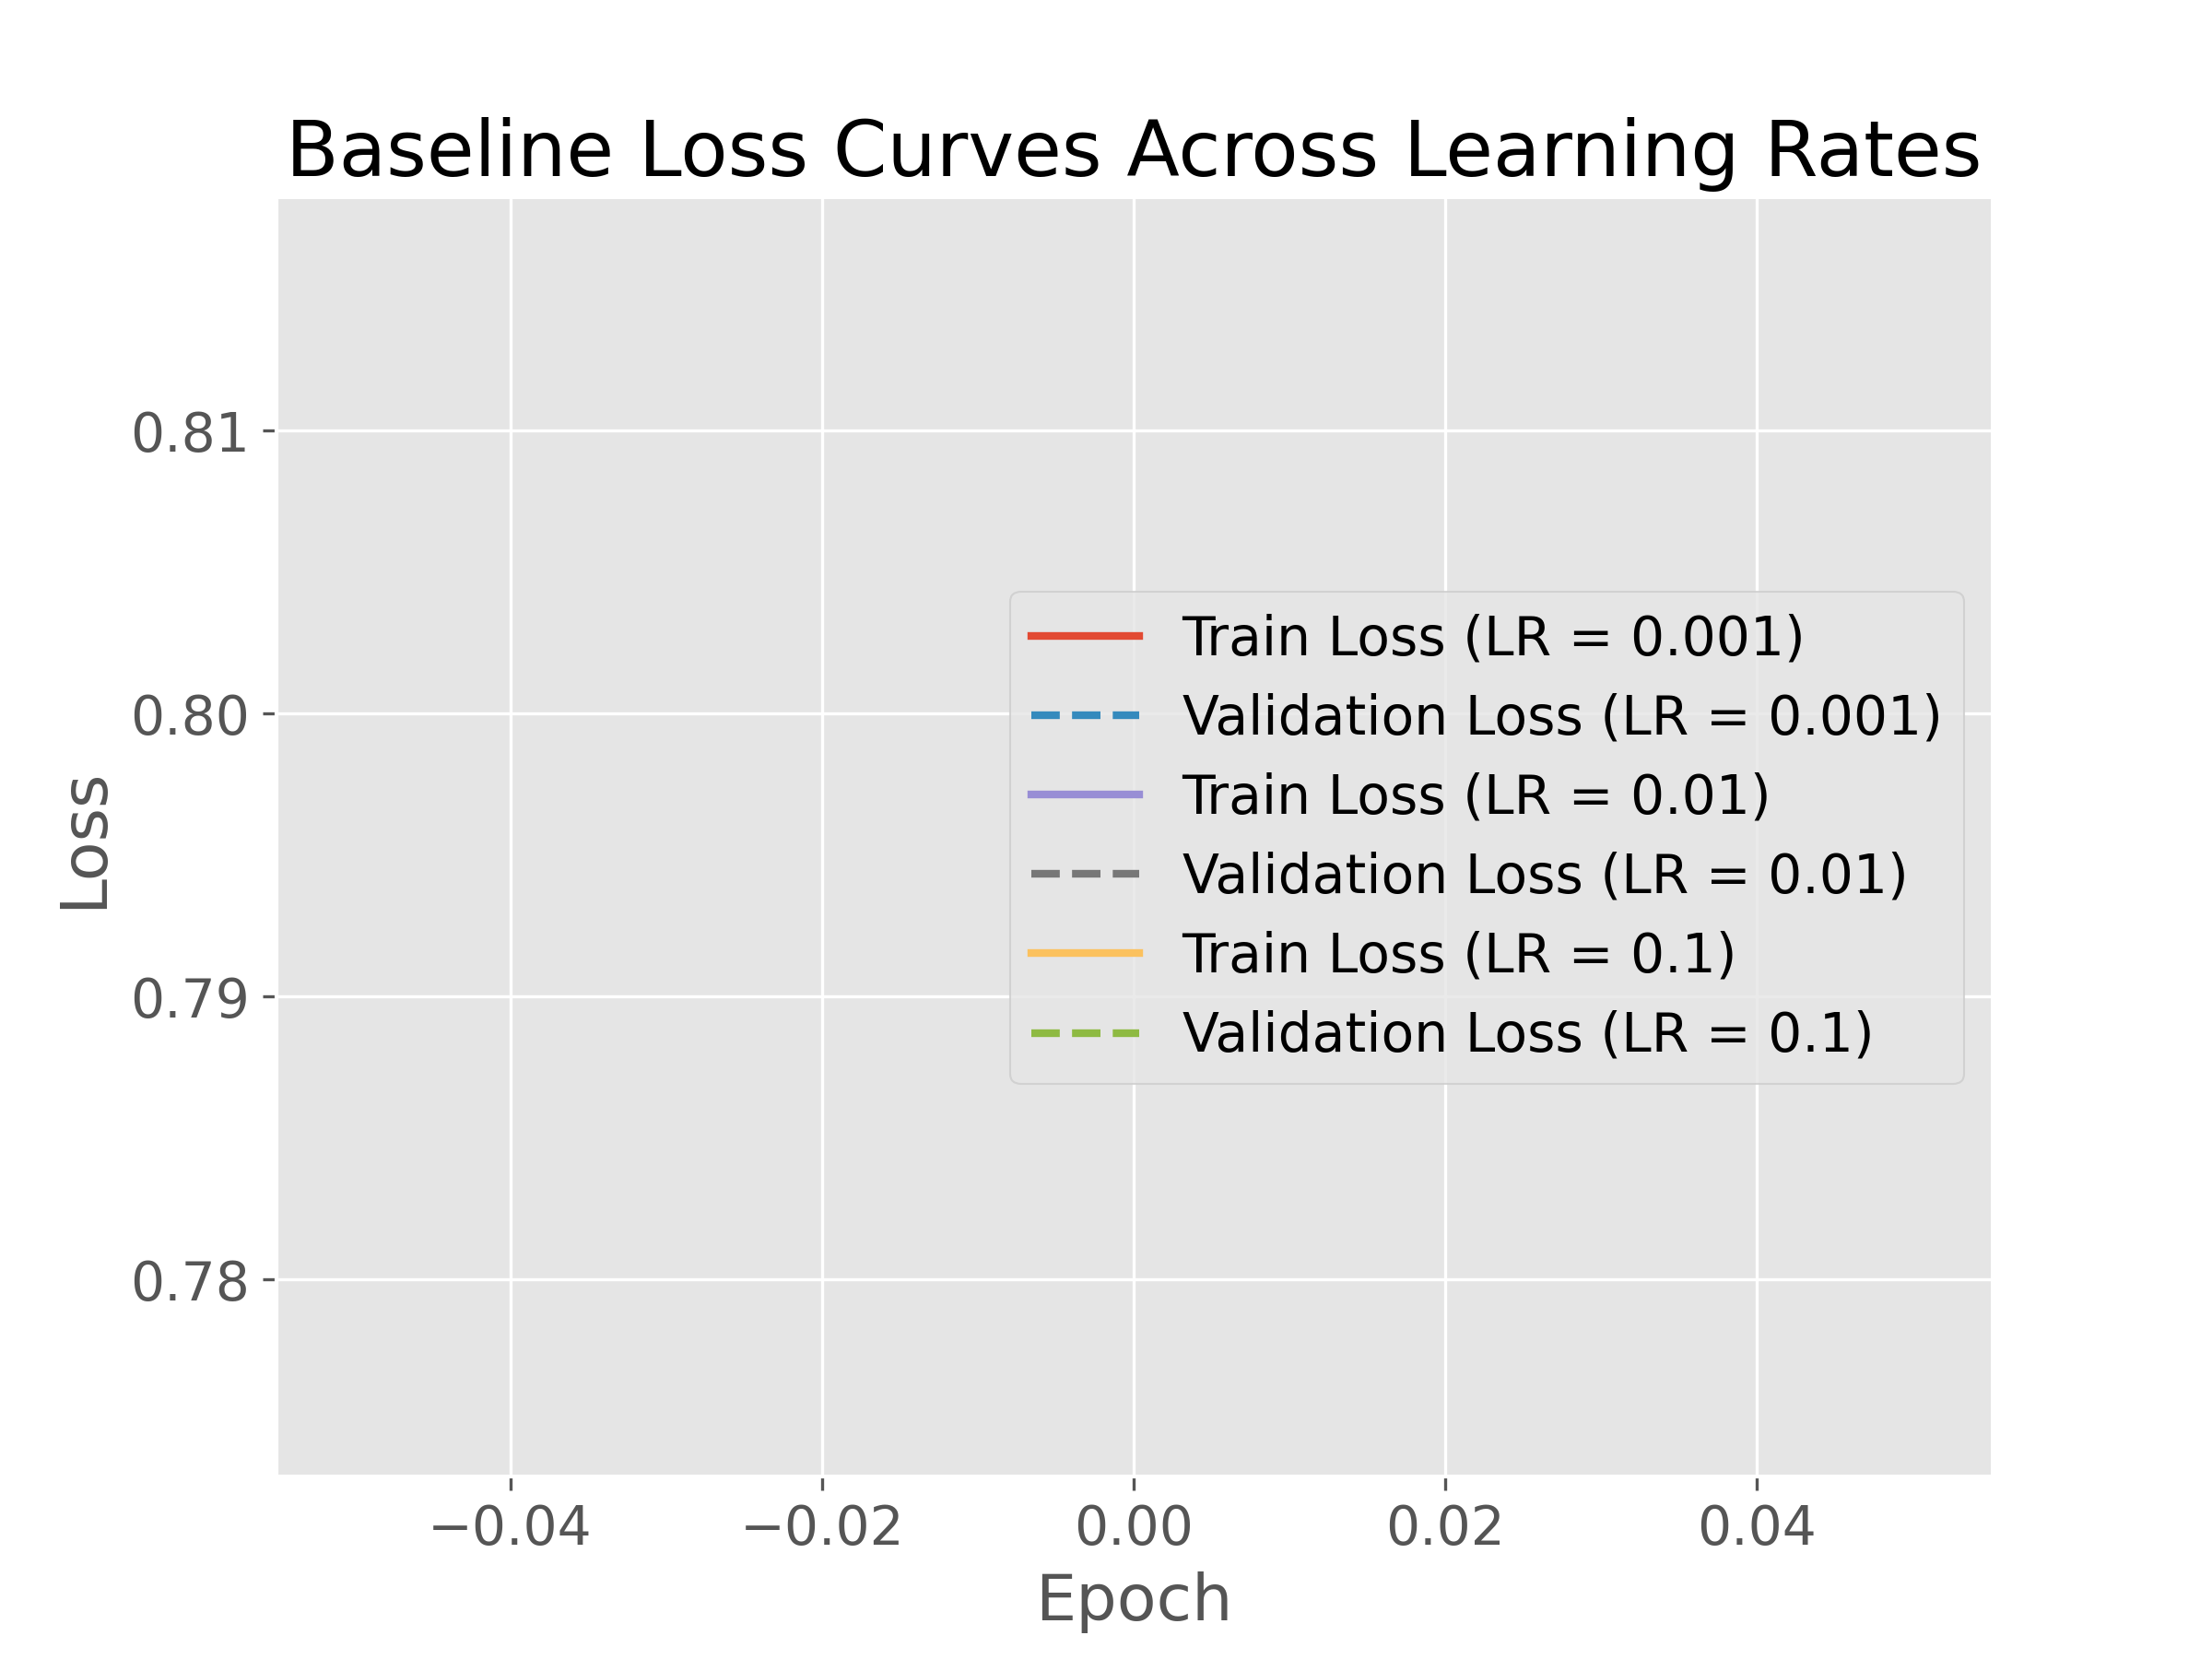
\includegraphics[width=0.6\textwidth]{img/Baseline Loss Curves.png}
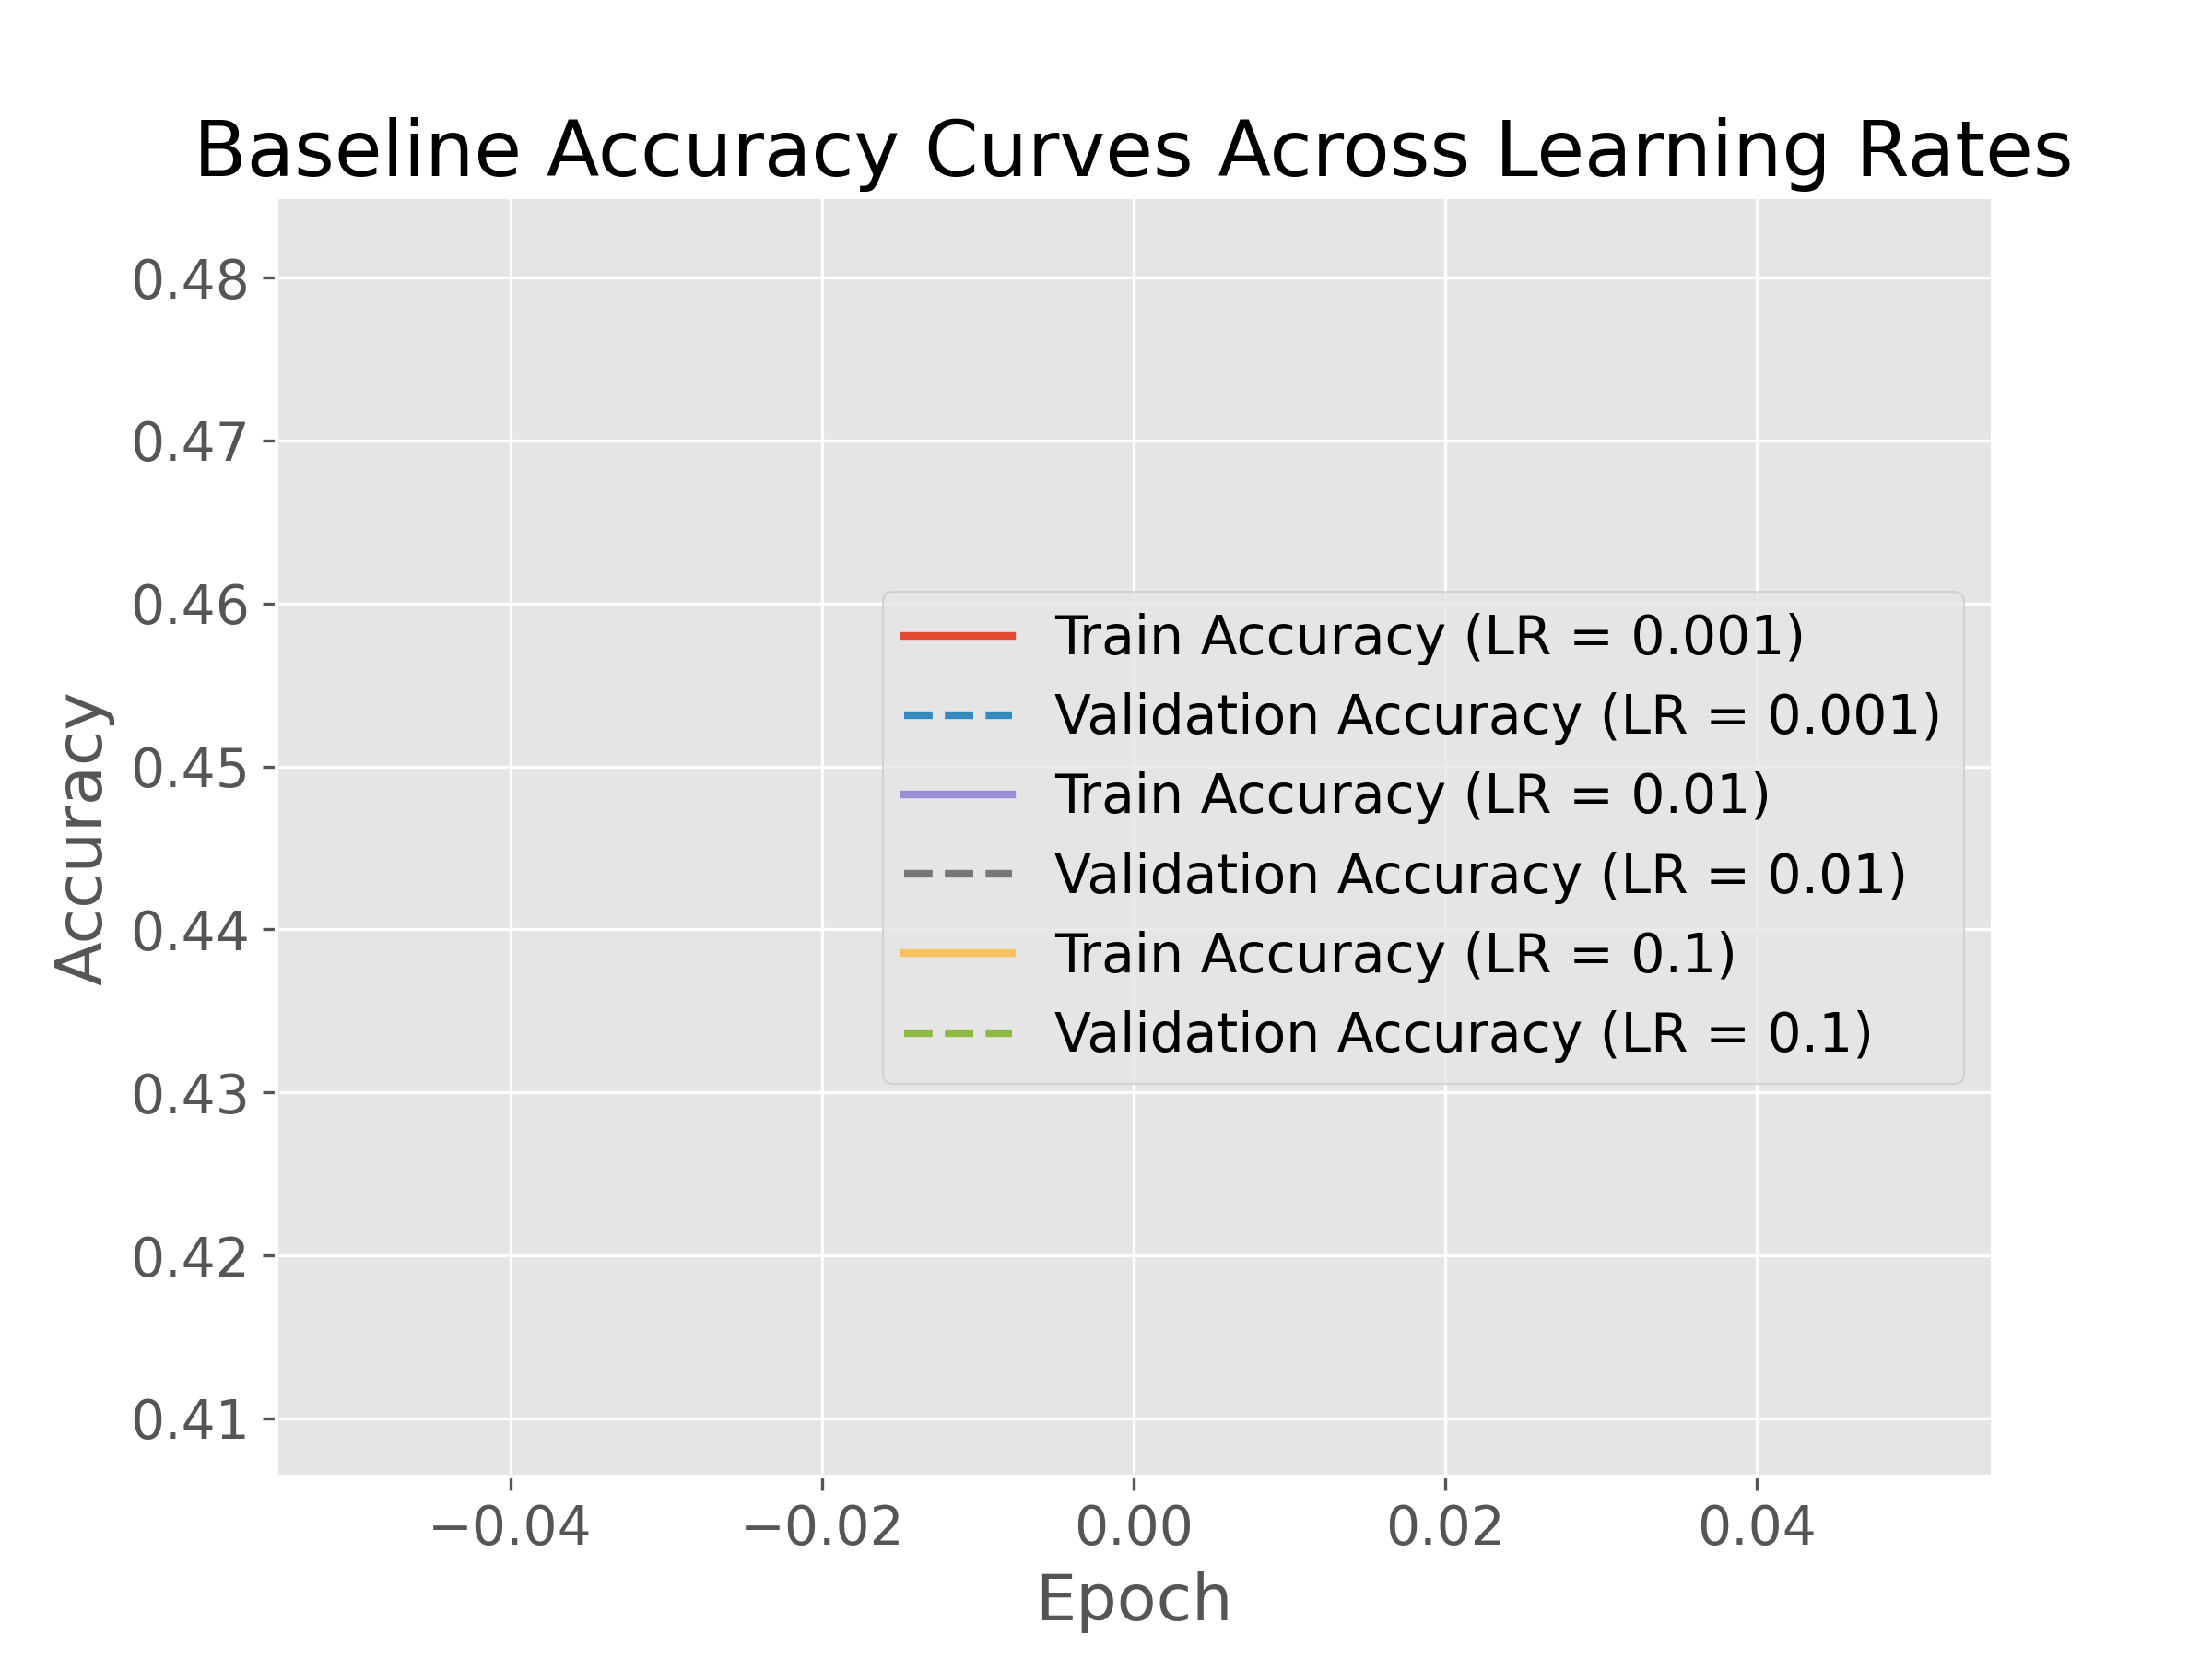
\includegraphics[width=0.6\textwidth]{img/Baseline Accuracy Curves.png}
\caption{Up: Baseline Loss Curves Across Learning Rates. Down: Baseline Accuracy Curves Across Learning Rates.}
\label{fig:baseline_loss}
\end{figure}

\begin{figure}[h!]
\centering
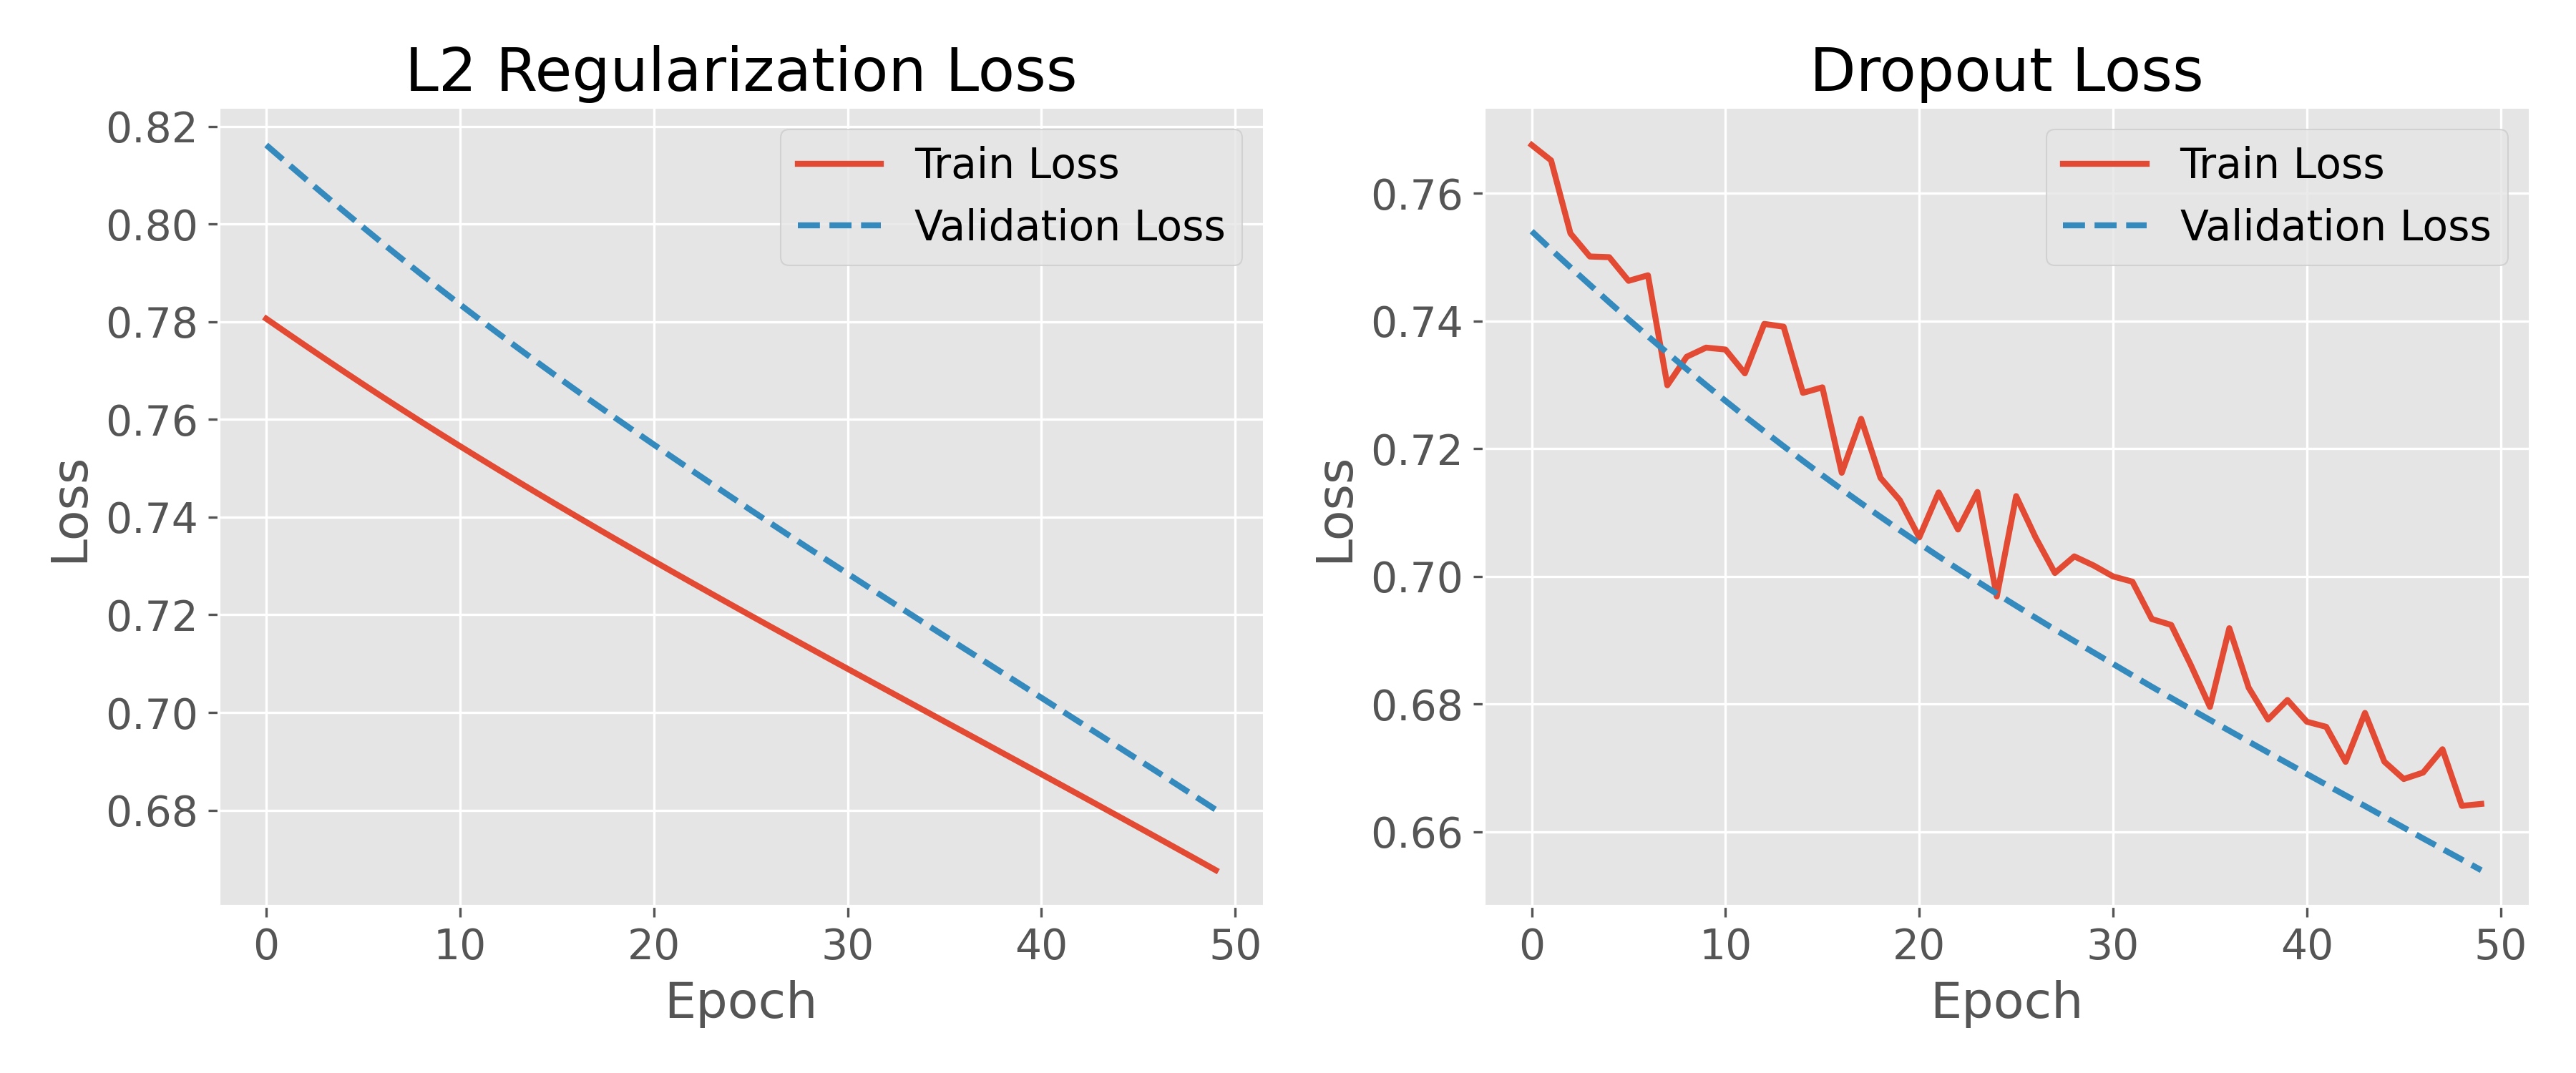
\includegraphics[width=0.79\textwidth]{img/Regularization Loss Curves.png}
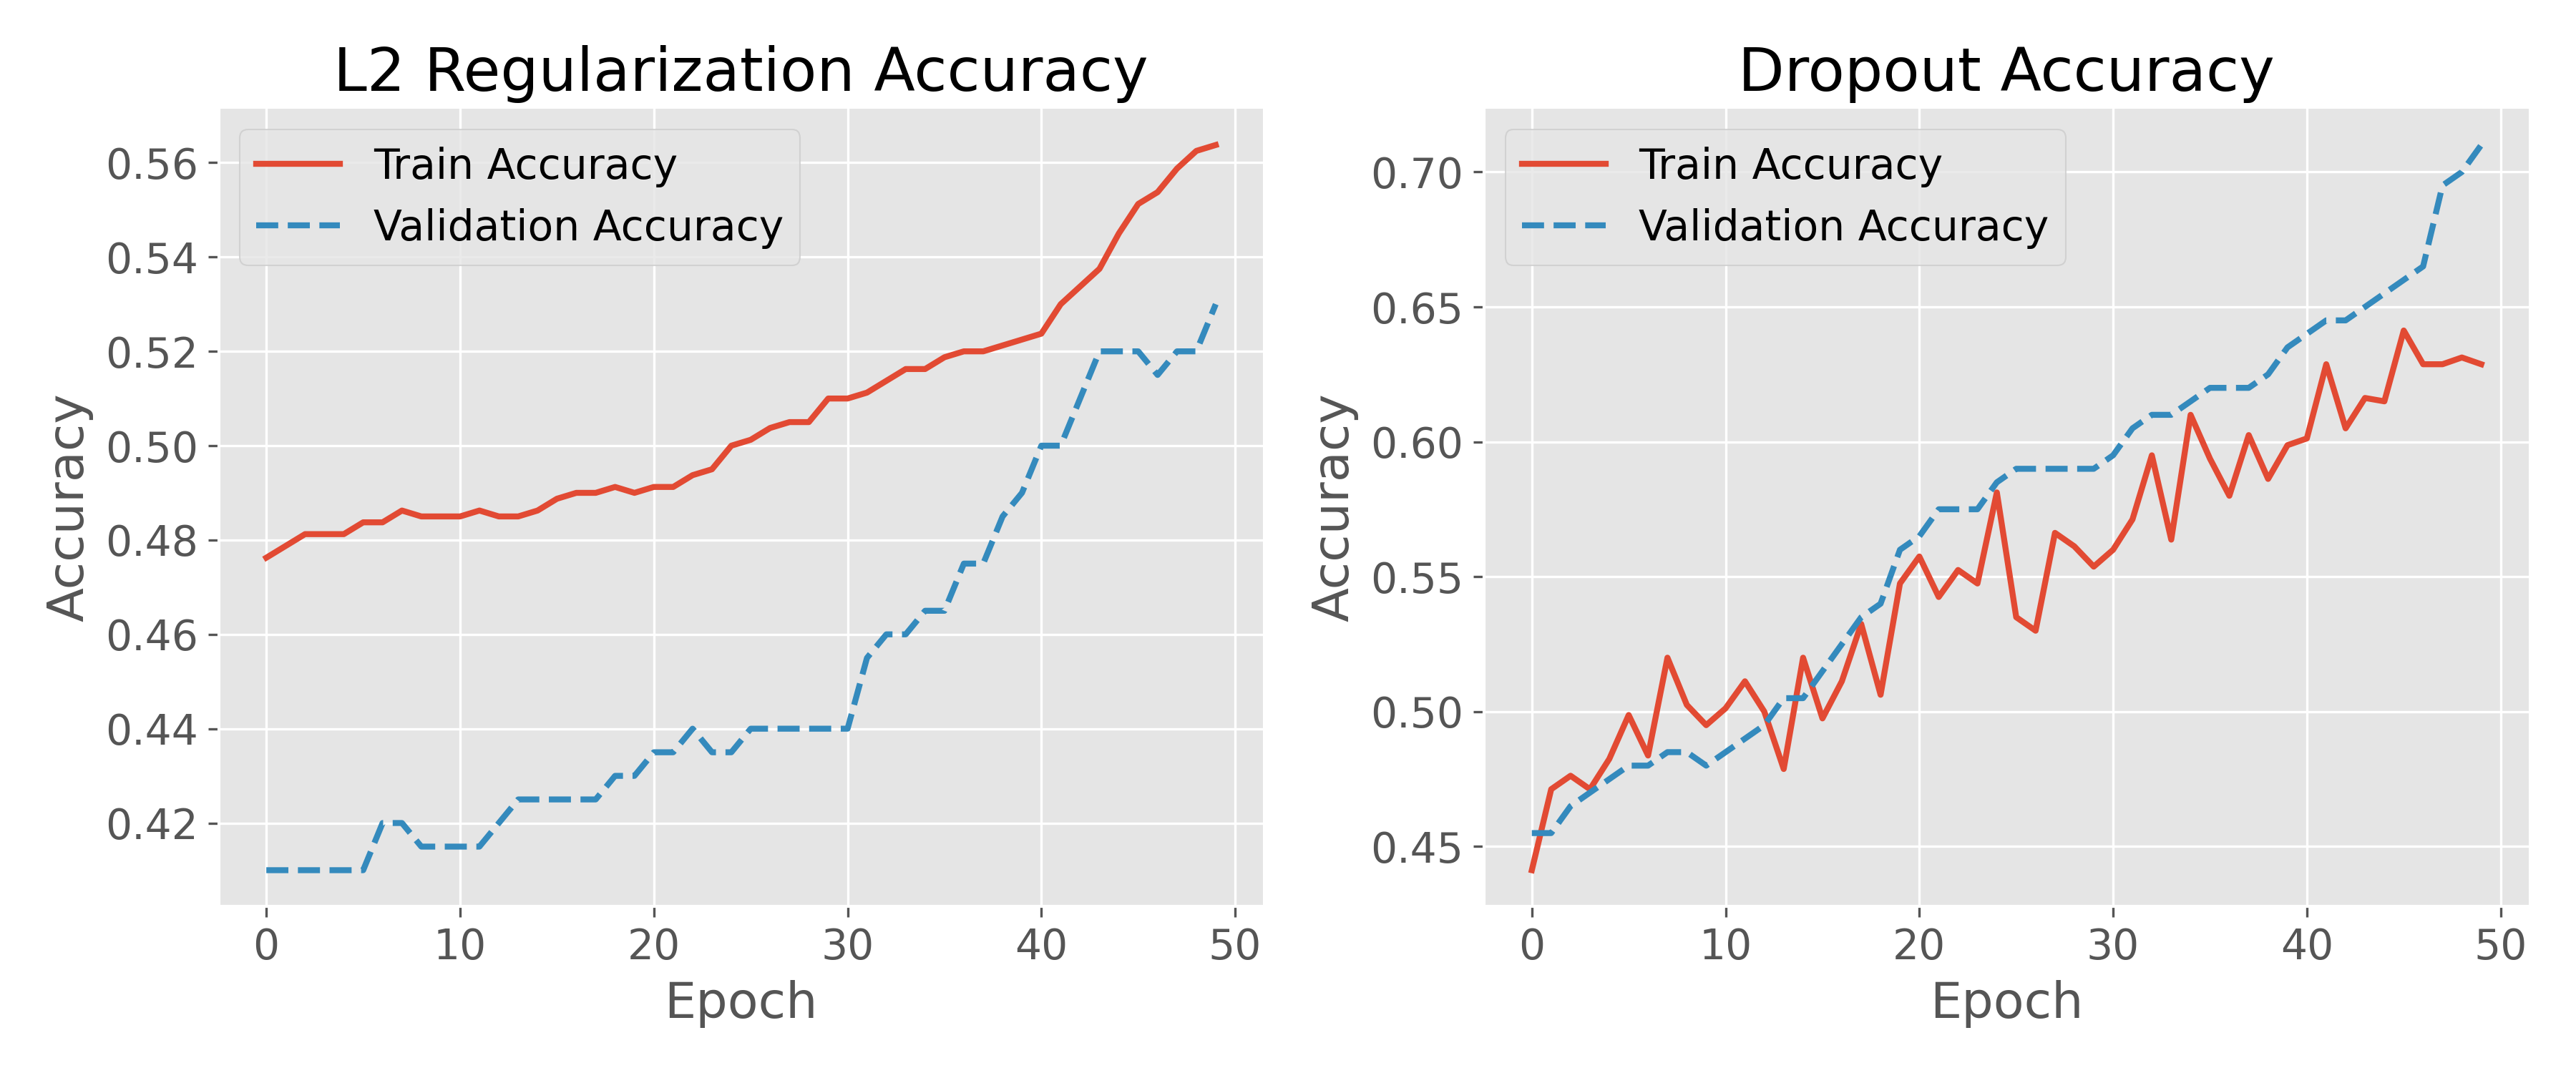
\includegraphics[width=0.79\textwidth]{img/Regularization Accuracy Curves.png}
\caption{Up: Regularization Loss Curves. Down: Regularization Accuracy Curves.}
\label{fig:regularization_curves}
\end{figure}

Figures \ref{fig:regularization_curves} and \ref{fig:training_epochs} illustrate the effects of regularization techniques and training epochs on model performance, further emphasizing the critical relationship between hyperparameter tuning and labor market dynamics.

\begin{figure}[h!]
\centering
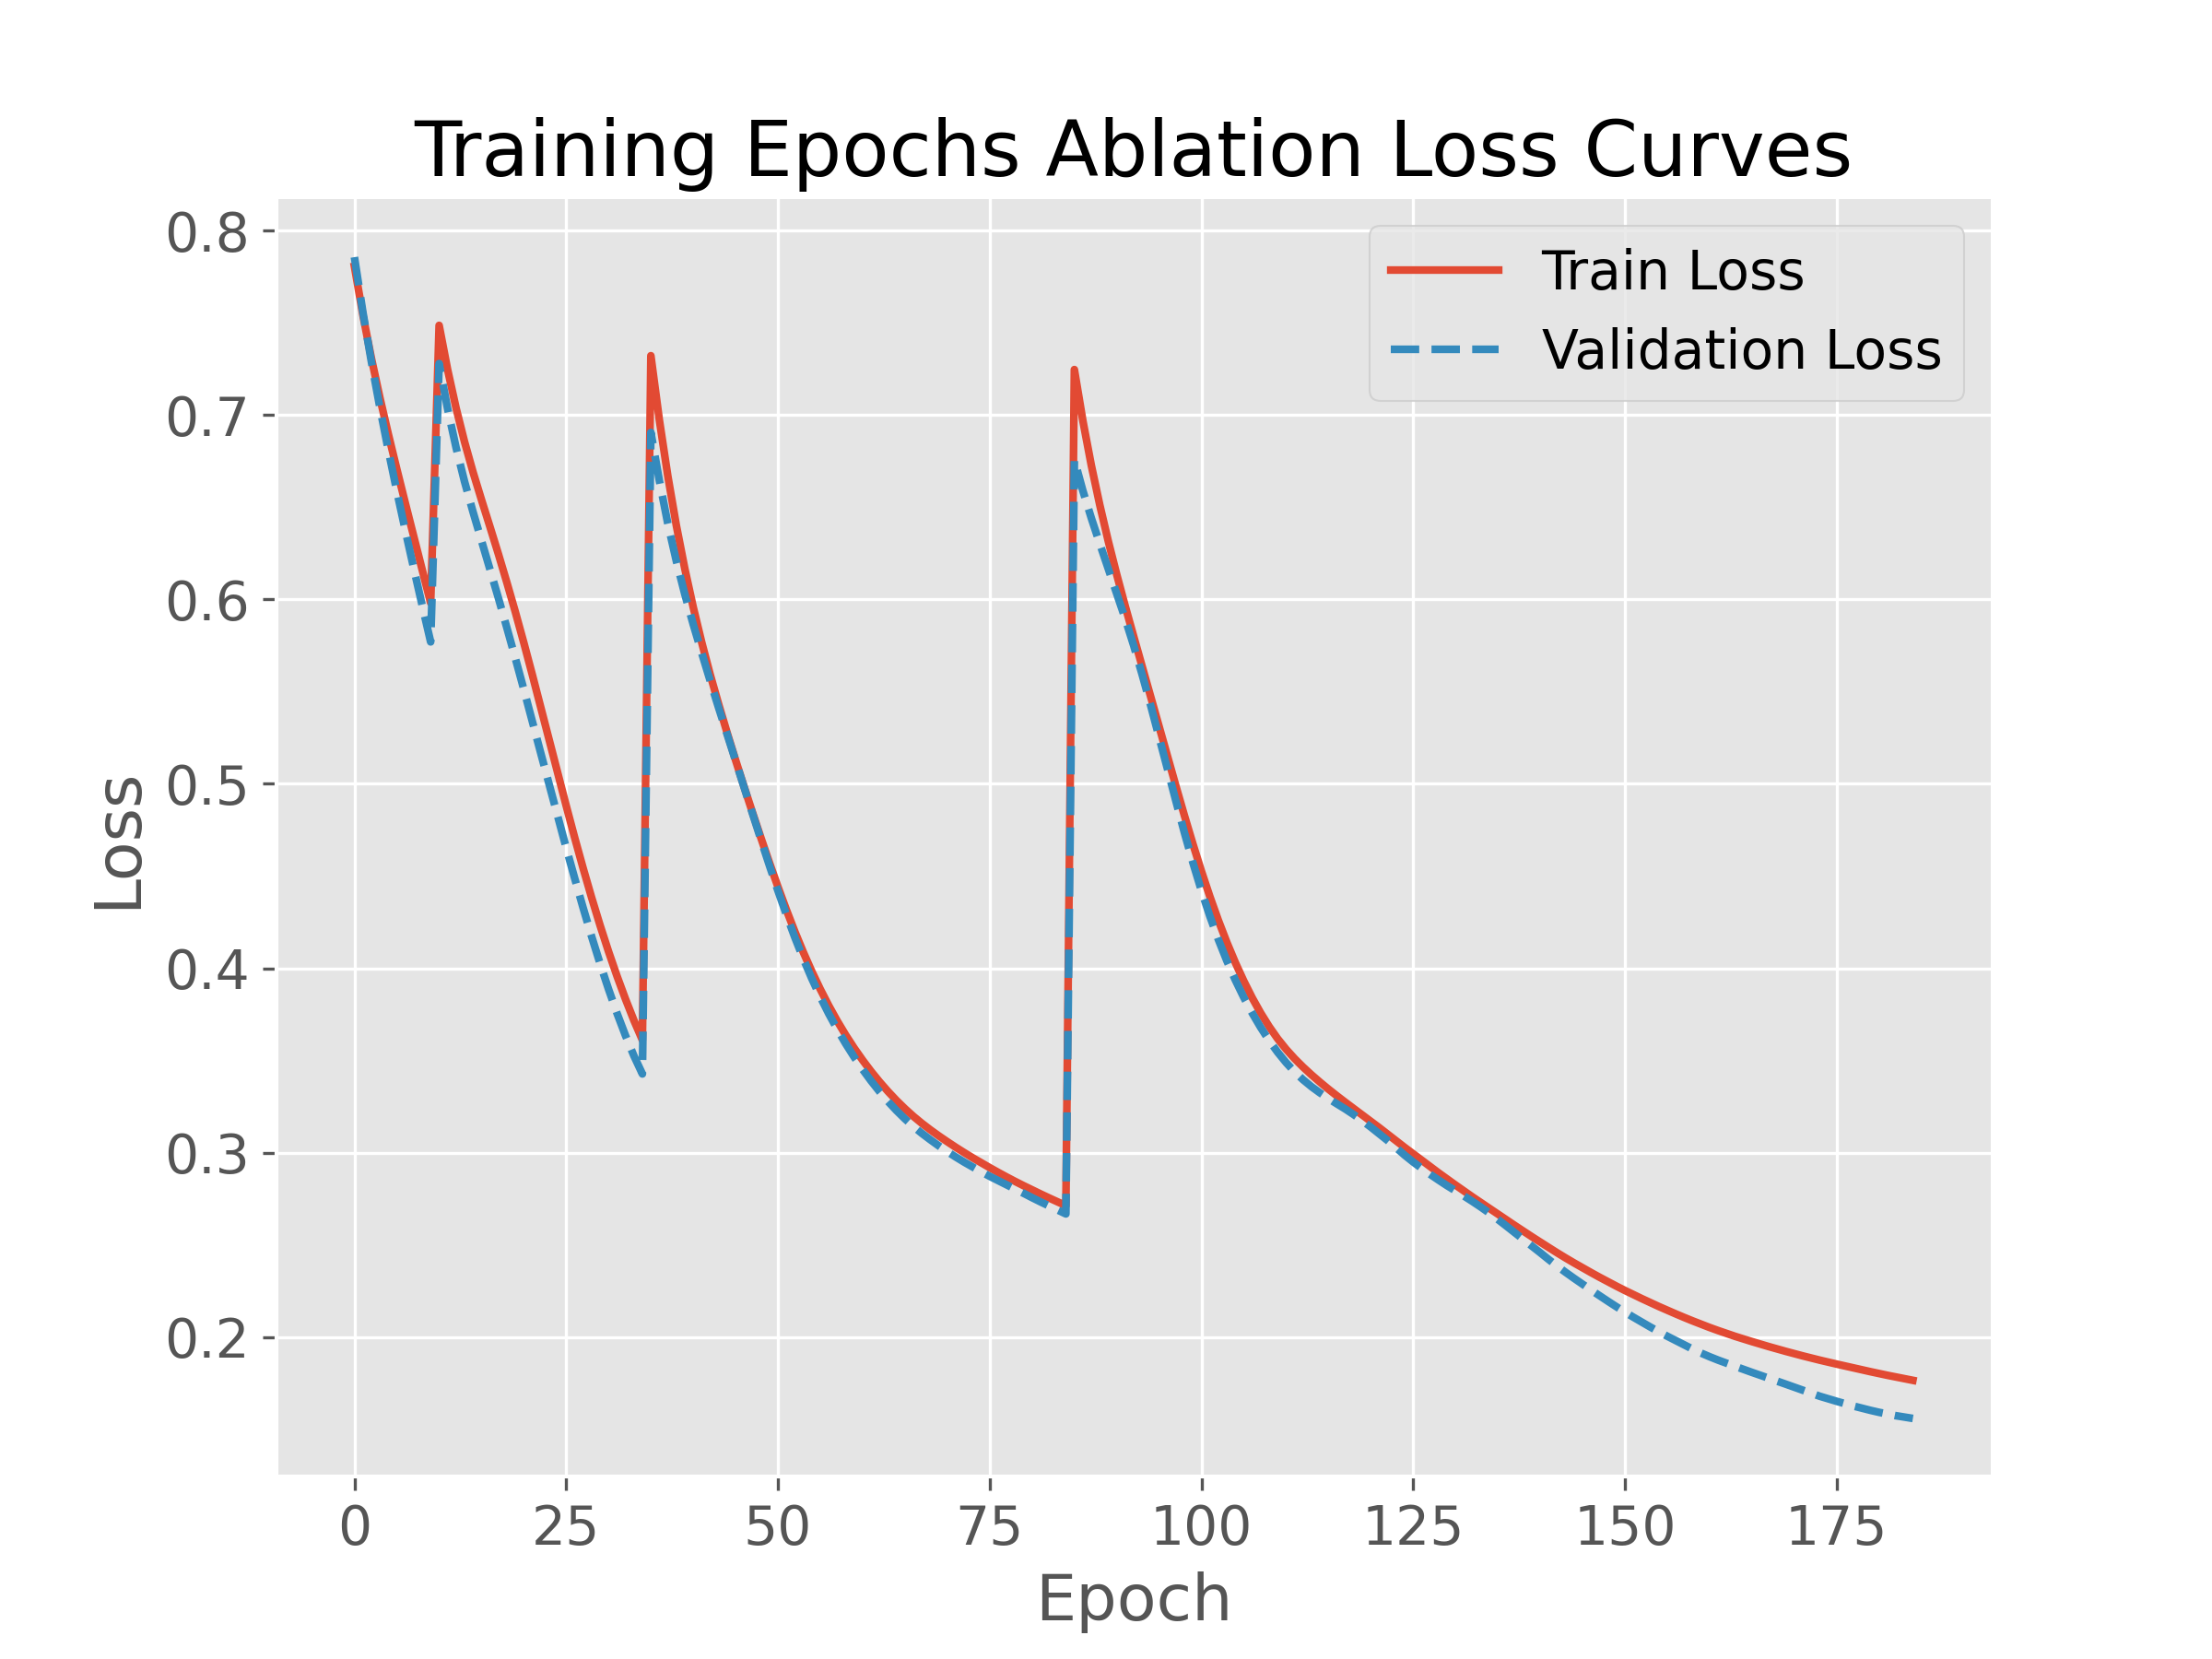
\includegraphics[width=0.49\textwidth]{img/Training Epochs Ablation Loss Curves.png}
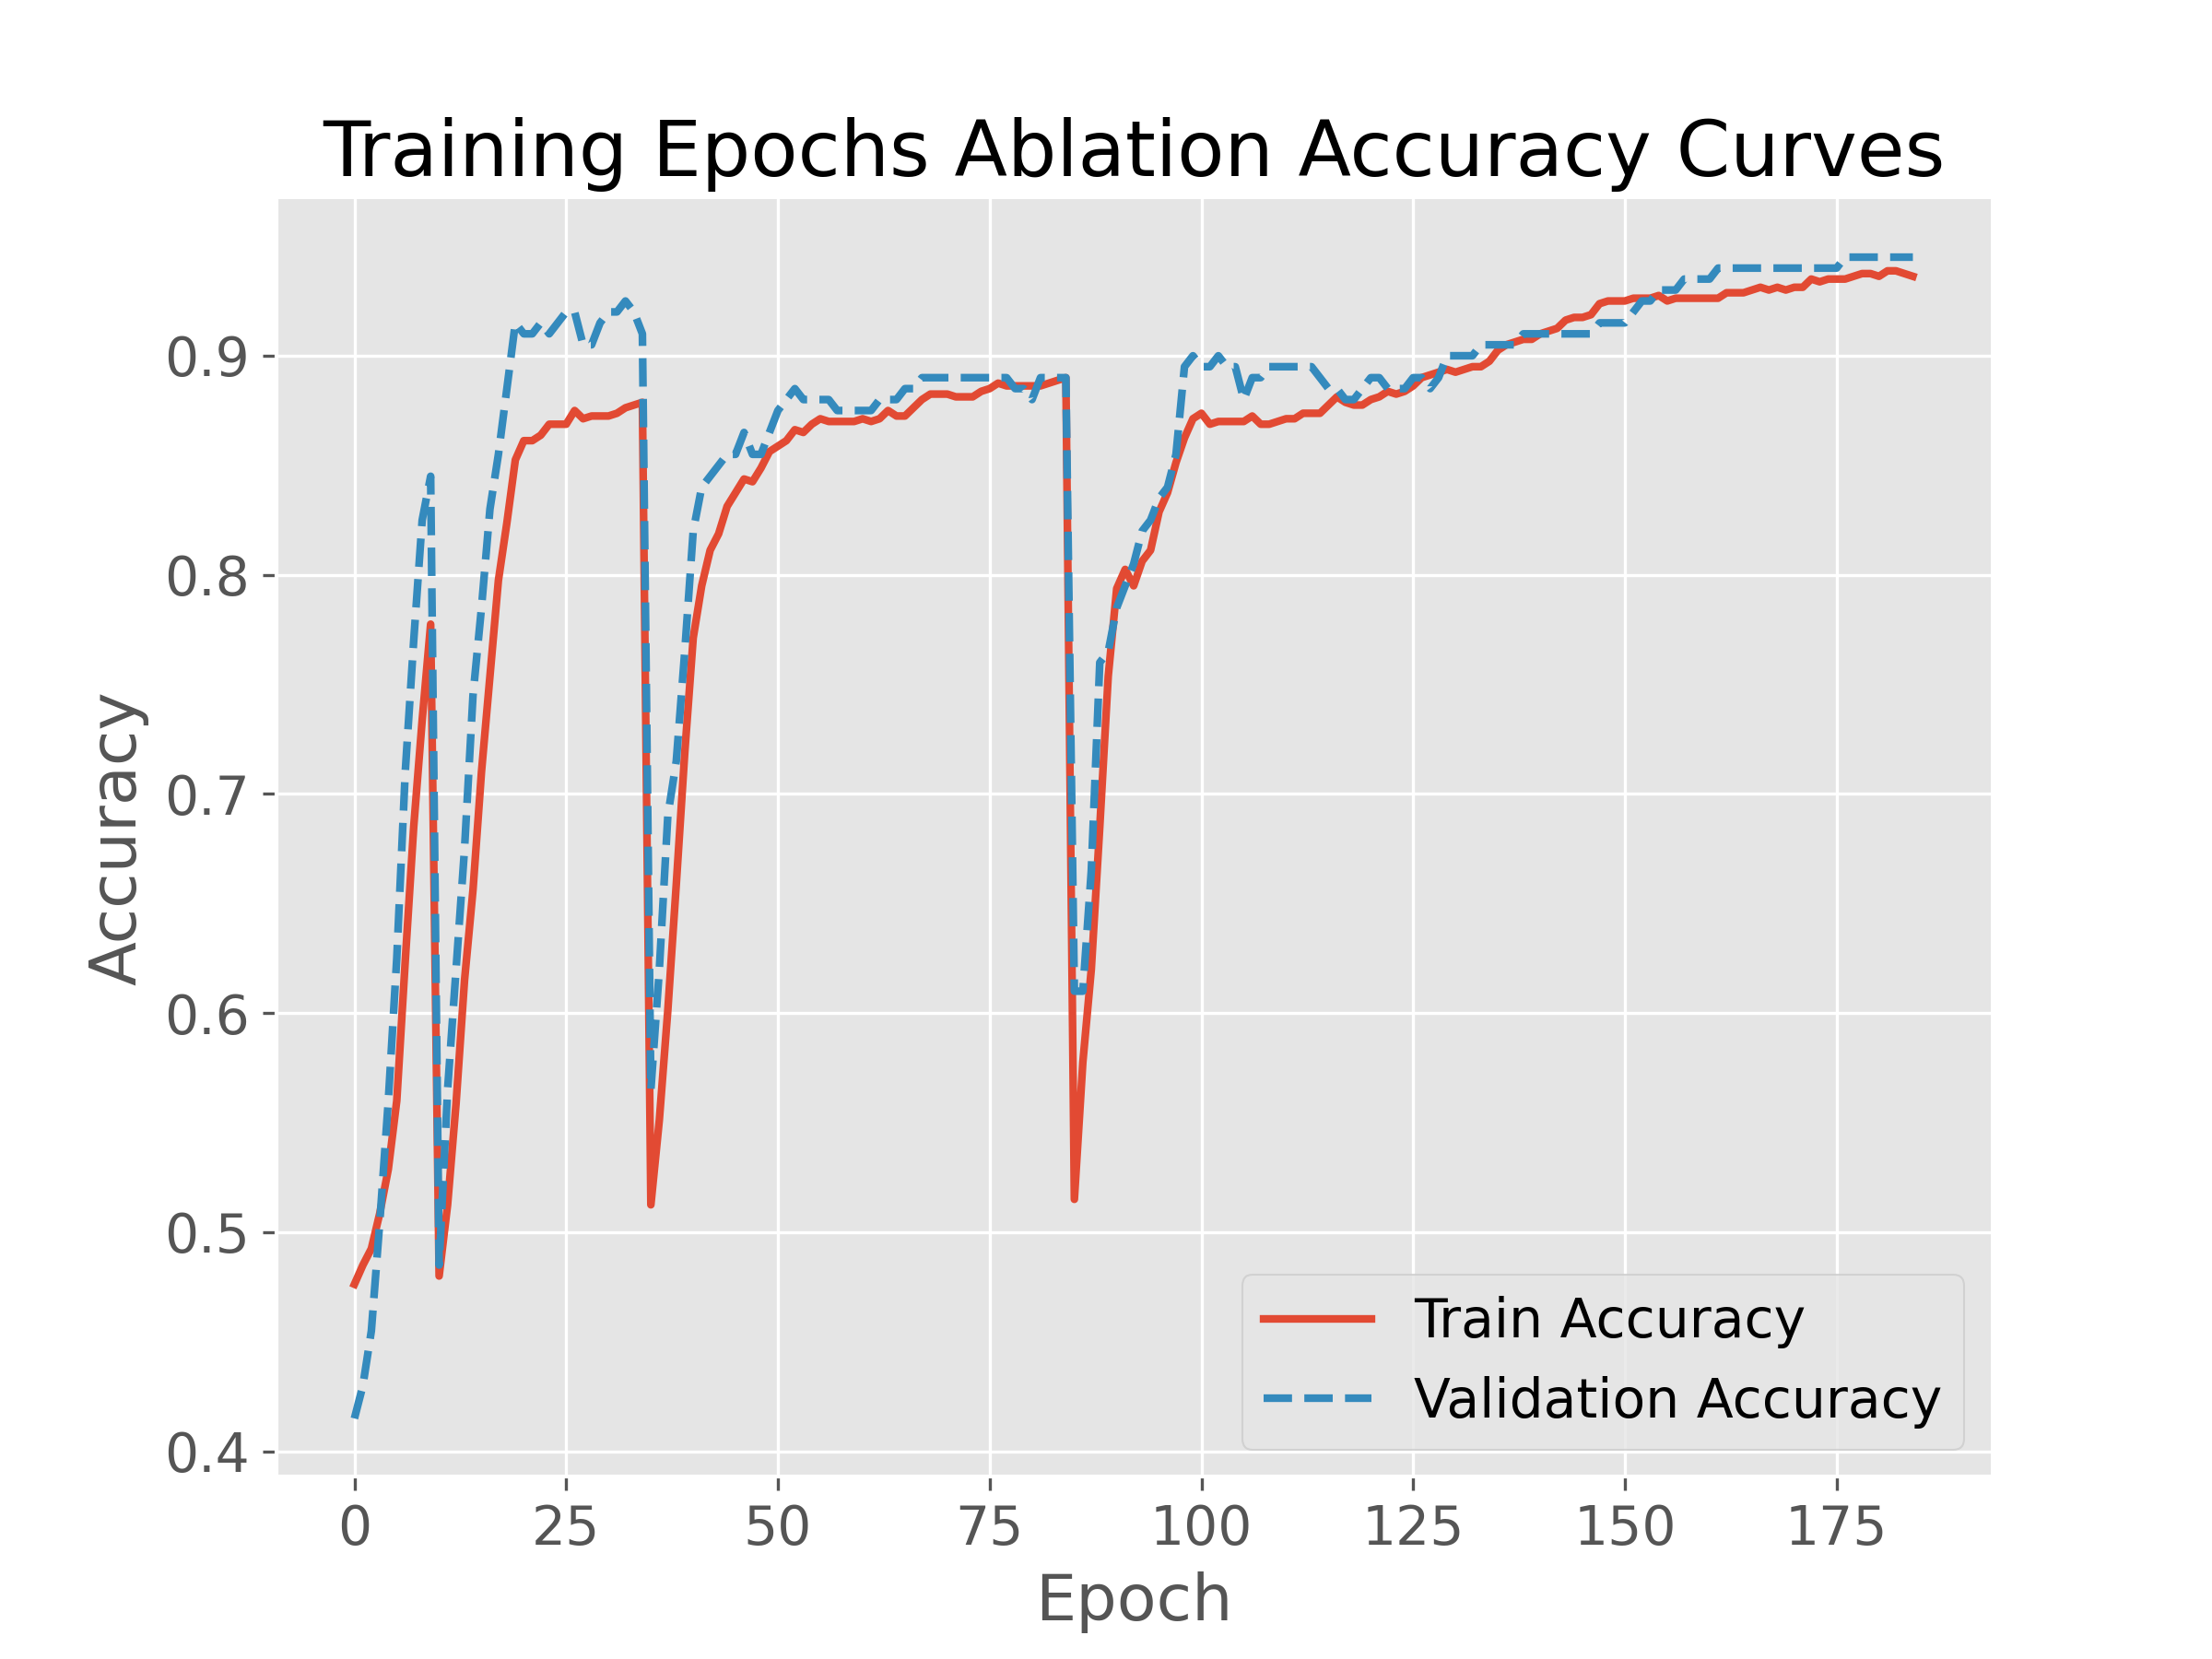
\includegraphics[width=0.49\textwidth]{img/Training Epochs Ablation Accuracy Curves.png}
\caption{Left: Training Epochs Ablation Loss Curves. Right: Training Epochs Ablation Accuracy Curves.}
\label{fig:training_epochs}
\end{figure}
The accuracy curves indicate significant variations across learning rates, yet the overall performance remains inadequate, reflecting the need for further model refinement. The loss curves also suggest that the model struggles to capture meaningful patterns, necessitating adjustments in training epochs and model architecture. 



\section{Conclusion}
Our findings highlight the urgent need for a pro-worker governance framework that addresses the systemic risks presented by AI in labor markets. By integrating worker rights and economic justice into governance strategies, we can create a more resilient labor market. Future work will focus on refining our experimental approach and further evaluating the effectiveness of proposed interventions. We believe that inclusive stakeholder dialogue is essential for shaping policies that safeguard against the adverse impacts of AI while promoting equitable growth.

\subsubsection*{Acknowledgments}




\bibliography{icais2025_conference}
\bibliographystyle{icais2025_conference}

% \appendix
% \section{Appendix}
% You may include other additional sections here.


\end{document}
